\documentclass[crop,tikz]{standalone}
\usetikzlibrary{tikzmark, bending, animations, fit, calc, positioning,arrows.meta}
\usepackage[tikz]{ocgx2}
\begin{document}

\begin{tikzpicture}[remember picture]
    \node (w) at (0,0) {\subnode[inner sep=2pt]{wd1}{Darüber} \subnode[inner sep=2.5pt]{wd2}{muss} \subnode[inner sep=1.5pt]{wd3}{nachgedacht} \subnode[inner sep=1.5pt]{wd4}{werden} \subnode[inner sep=2.5pt]{wd5}{.}};

    % muss
    \draw[-Stealth] ($(wd2.north) + (2pt, 0)$) to [bend left=50] node [above, scale=0.5] {\(\mathrm{C}_{1}\)} ($(wd4.north) + (2pt, 0)$);
    \draw[-Stealth] ($(wd2.north) + (2pt, 0)$) to [bend left=80] node [above, scale=0.5] (s2) {\(\mathrm{S}_{2}\)} (wd5.north);

    % werden
    \draw[-Stealth] ($(wd4.north) - (2pt, 0)$) to [bend right=30] node [above, scale=0.5] {VP} ($(wd3.north) + (2pt, 0)$);

    % nachgedacht
    \draw[-Stealth] ($(wd3.north) - (2pt, 0)$) to [bend right=60] node [above, scale=0.5] {VP} (wd1.north);

    \node[scale=0.5] (root) at ({$(wd2) - (2pt, 0)$} |- s2) {\texttt{root}};
    \draw[-Stealth] (root.south) -- (root |- wd2.north);
\end{tikzpicture}

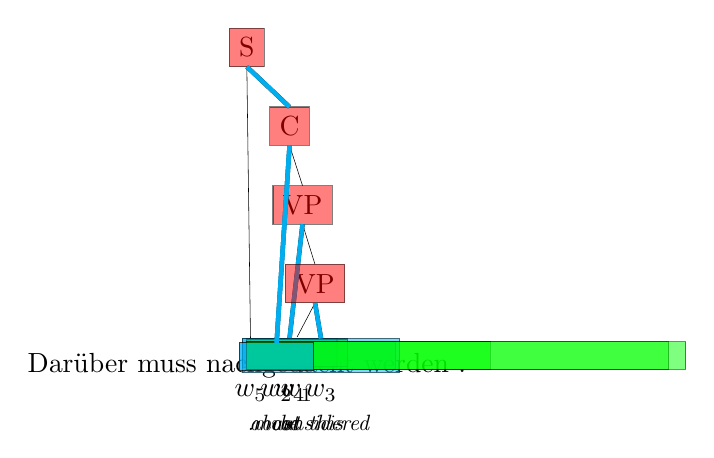
\begin{tikzpicture}[remember picture]
    \node[inner sep=0, text depth=0] (w) {\subnode[inner sep=0]{s-yld}{\subnode[inner sep=0]{c-yld}{\subnode[inner sep=0]{vptop-left}{\subnode[inner sep=0]{vpbot-left}{\subnode[inner sep=2pt]{w1}{Darüber}}} \subnode[inner sep=2.5pt]{w2}{muss} \subnode[inner sep=0]{vptop-right}{\subnode[inner sep=0]{vpbot-right}{\subnode[inner sep=1.5pt]{w3}{nachgedacht}} \subnode[inner sep=1.5pt]{w4}{werden}}} \subnode[inner sep=2.5pt]{w5}{.}}};

    \foreach \n/\english in {1/about this,2/must,3/considered,4/be,5/.} \node[below=1ex of {w\n |- w.south}, inner sep=0, align=center] {\(w_{\n}\) \\[0ex] \scalebox{0.8}{\textit{\english}}};
    
    % \coordinate (s) at ({barycentric cs:w1=1,w2=1,w3=1,w4=1} |- {barycentric cs:w=1,vroot=4});
    
    \node[switch ocg=const-s] (vroot) at ($(w) + (0, 4cm)$)  {S};
    \node[switch ocg=const-c] (s) at ({barycentric cs:w1=1,w2=3,w3=1,w4=1} |- {barycentric cs:w=1,vroot=3}) {C};
    \node[switch ocg=const-vptop] (vp1) at ({barycentric cs:w1=1,w3=1,w4=1} |- {barycentric cs:w=2,vroot=2}) {VP};
    \node[switch ocg=const-vpbot] (vp2) at ({barycentric cs:w1=1,w3=3} |- {barycentric cs:w=3,vroot=1}) {VP};

    \draw[very thin] (vroot.south) -- (w5.north);
    \draw[ultra thick] (vroot.south) -- (s.north);
    \draw[ultra thick] (s.south) -- (w2.north);
    \draw[very thin] (s.south) -- (vp1.north);
    \draw[ultra thick] (vp1.south) -- (w4.north);
    \draw[very thin] (vp1.south) -- (vp2.north);
    \draw[very thin] (vp2.south) -- (w1.north);
    \draw[ultra thick] (vp2.south) -- (w3.north);

    % vptop
    \begin{scope}[ocg={ref=const-vptop, status=invisible, opts={radiobtngrp=const}}]
        \node[draw, fit=(vp1), fill=red, inner sep=0, opacity=0.5] {};
        \node[draw, fit=(vptop-right), fill=green, inner sep=0, minimum height=1em, opacity=0.5] {};
        \node[draw, fit=(vptop-left), fill=green, inner sep=0, minimum height=1em, opacity=0.5] {};
        \node[draw, fit=(w4), fill=cyan, inner sep=0, minimum height=1em, opacity=0.5] {};
        \draw[ultra thick, cyan] (vp1.south) -- (w4.north);
    \end{scope}

    % vpbot
    \begin{scope}[ocg={ref=const-vpbot, status=invisible, opts={radiobtngrp=const}}]
        \node[draw, fit=(vp2), fill=red, inner sep=0, opacity=0.5] {};
        \node[draw, fit=(vpbot-right), fill=green, inner sep=0, minimum height=1em, opacity=0.5] {};
        \node[draw, fit=(vpbot-left), fill=green, inner sep=0, minimum height=1em, opacity=0.5] {};
        \node[draw, fit=(w3), fill=cyan, inner sep=0, minimum height=1em, opacity=0.5] {};
        \draw[ultra thick, cyan] (vp2.south) -- (w3.north);
    \end{scope}

    % c-yld
    \begin{scope}[ocg={ref=const-c, status=invisible, opts={radiobtngrp=const}}]
        \node[draw, fit=(s), fill=red, inner sep=0, opacity=0.5] {};
        \node[draw, fit=(c-yld), fill=green, inner sep=0, minimum height=1em, opacity=0.5] {};
        \node[draw, fit=(w2), fill=cyan, inner sep=0, minimum height=1em, opacity=0.5] {};
        \draw[ultra thick, cyan] (s.south) -- (w2.north);
    \end{scope}

    % s-yld
    \begin{scope}[ocg={ref=const-s, status=invisible, opts={radiobtngrp=const}}]
        \node[draw, fit=(vroot), fill=red, inner sep=0, opacity=0.5] {};
        \node[draw, fit=(s-yld), fill=green, inner sep=0, minimum height=1em, opacity=0.5] {};
        \node[draw, fit=(w2), fill=cyan, inner sep=0, minimum height=1em, opacity=0.5] {};
        \draw[ultra thick, cyan] (vroot.south) -- (s.north);
        \draw[ultra thick, cyan] (s.south) -- (w2.north);
    \end{scope}
\end{tikzpicture}

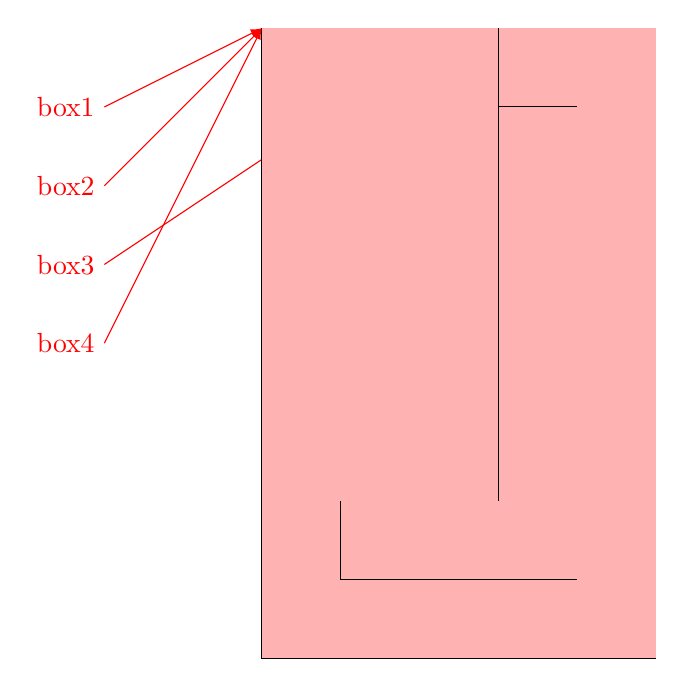
\begin{tikzpicture}[yscale=-1,>=latex]
    \foreach \a/\b/\c/\d/\desc [count=\j] in {
        0/0/5/8/box1,
        0/0/2/4/box2,
        1/1/4/7/box3,
        0/0/3/6/box4
    }{
        \path (-2,0) ++(0,\j) coordinate (A);
        \draw (\a,\b) rectangle (\c,\d);
        \begin{scope}[ocg={ref=box\j,status=invisible,opts={radiobtngrp=myBoxes}}]
            \fill[red!30] (\a,\b) rectangle (\c,\d);
        \end{scope}
        \draw[<-,red] (\a,\b) -- (A) node[anchor=east,pos=1,switch ocg=box\j] {\desc};
    }
    \end{tikzpicture}
\end{document}